%!TEX program = lualatex
\documentclass[border=0mm,11pt]{standalone}
%\usepackage{color}
%\usepackage{tikz}
\usepackage[T1]{fontenc}
\usepackage[sc]{mathpazo}
\usepackage{tikz-feynman}
\tikzfeynmanset{compat=1.1.0}


\begin{document}

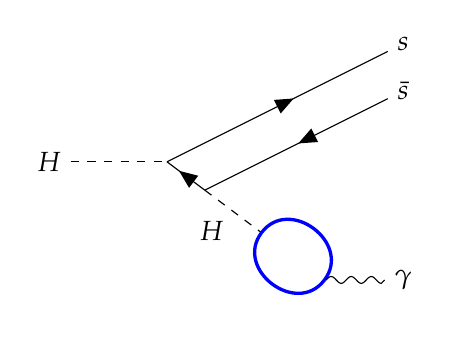
\begin{tikzpicture}[]
    \begin{feynman}
    \vertex (h) {$H$};
    \vertex [right=of h, xshift=0.0cm, yshift=-0.0cm] (cent);
    \vertex [right=of h, xshift=3.0cm, yshift=1.5cm] (b) {$s$};
    \vertex [right=of h, xshift=3.0cm, yshift=0.9cm] (e) {$\bar{s}$};
    \vertex [right=of h, xshift=0.48cm, yshift=-0.36cm] (middle);
    \vertex [right=of h, xshift=1.2cm, yshift=-0.9cm] (middle2);
    \vertex [right=of h, xshift=2.0cm, yshift=-1.5cm] (middle3);
    \vertex [right=of h, xshift=3.0cm, yshift=-1.5cm] (f) {$\gamma$};

    %\node [dot] at (cent) {};
    \diagram* {
    (h) -- [scalar] (cent),
    (b) -- [anti fermion] (cent) -- [with reversed arrow=0.7] (middle) -- [with reversed arrow=0.6] (e),
    (middle) -- [scalar, edge label'=\(H\)] (middle2),
    (middle2) -- [blue, very thick, half left] (middle3) -- [blue, very thick, half left] (middle2),
    (middle3) -- [photon] (f),
    
    };
    \end{feynman}
\end{tikzpicture}

\end{document}